\documentclass[12pt]{report}
\usepackage[francais]{babel}
\usepackage{latexsym}

\usepackage{graphicx}
\usepackage{enumerate}

% Les paquetage suivants peuvent �tre utiles. Les d�commenter au besoin
% \usepackage{amssymb}
% \usepackage{amsmath}

\usepackage[latin1]{inputenc} % Pour pouvoir taper les accent directement et non pas passer par \'


\setlength{\oddsidemargin}{-0,4in} \topmargin -12,0mm
 \textheight 24,5cm \textwidth 17,8cm



\begin{document}
	
\title{IFT-4001 (Hiver 2016) Travail pratique}
\date{21 f�vrier 2016}
\author{Vincent Beaudoin (111 103 778)\\Alexandre Picard-Lemieux (111 103 625)}

\maketitle
\newpage

\textbf{\Large Premier probl�me}\\

On d�clare une variable pour chaque �l�ment de la matrice. Ainsi, la variable $X_{ij}$ repr�sente la valeur inscrite � la ligne $i$ et la colonne $j$ pour $1 \leq i \leq 4$ et $1 \leq j \leq n$. Ces quatre lignes forme les quatres longues faces d'un rectangle. $n$ repr�sente le nombre de cube que forme ce rectangle. Le domaine de chaque variable est l'ensemble des entiers entre 1 et n, c'est-�-dire les couleurs. Nous avons les tuples pour $n = 4$ qui ont �t� d�finis dans le probl�me:\\

$T_1$:
\begin{tabular}{ |c|c| } 
	\hline
	x & y \\
	\hline
	JAUNE & VERT \\
	VERT & JAUNE \\
	ROUGE & BLEU \\
	BLEU & ROUGE \\
	VERT & ROUGE \\
	ROUGE & VERT \\
	\hline
\end{tabular}
\quad
$T_2$:
\begin{tabular}{ |c|c| } 
	\hline
	x & y \\
	\hline
	VERT & VERT \\
	ROUGE & BLEU \\
	BLEU & ROUGE \\
	JAUNE & BLEU \\
	BLEU & JAUNE \\
	\hline
\end{tabular}

$T_3$:
\begin{tabular}{ |c|c| } 
	\hline
	x & y \\
	\hline
	BLEU & ROUGE \\
	ROUGE & BLEU \\
	JAUNE & JAUNE \\
	JAUNE & VERT \\
	VERT & JAUNE \\
	\hline
\end{tabular}
\quad
$T_4$:
\begin{tabular}{ |c|c| } 
	\hline
	x & y \\
	\hline
	JAUNE & ROUGE \\
	ROUGE & JAUNE \\
	ROUGE & VERT \\
	VERT & ROUGE \\
	BLEU & JAUNE \\
	JAUNE & BLEU \\
	\hline
\end{tabular}

Pour chaque ligne $i$, nous avons une contrainte $X_{ij} \neq X_{ik}$ pour chacune des $\frac{n(n-1)}{2}$ paires de variables.

\begin{equation}
X_{ij} \neq X_{ik} \quad \forall 1 \leq j, k \leq n
\end{equation}

Pour chaque colonne j, nous avons ces contraintes.

\begin{equation}
Tableau(X_{ij}, X_{(i+2)j}, T_j) \quad \forall 1 \leq i \leq 2
\end{equation}

\begin{equation}
ifThen(X_{ij} = X_{(i+1)j}, X_{(i+2)j} \neq X_{(i+3)j})
\end{equation}

\begin{equation}
ifThen(X_{ij} = X_{(i+3)j}, X_{(i+1)j} \neq X_{(i+2)j})
\end{equation}

Nous avons donc $4n \in \Theta(n)$ variables. Chaque variable a $n$ valeurs dans son domaine pour un total de $\Theta(n^2)$ valeurs. Nous avons $4$ contraintes de type (1), $2n$ contraintes de type (2), $n$ contraintes de type (3) et $n$ contraintes de type (4). Nous avons donc au total $4 + 2n + n + n \in \Theta(n)$ contraintes. Chaque contrainte tableau poss�de $6 \in \Theta(1)$ entr�es.\\

La solution retourn�e par le solveur Choco 3:\\
VERT  ROUGE  JAUNE  BLEU  \\
JAUNE  BLEU  ROUGE  VERT  \\
ROUGE  BLEU  VERT  JAUNE  \\
VERT  JAUNE  BLEU  ROUGE  \\

Le temps requis au solveur pour trouver la solution est de 0,045 secondes. Le nombre de retours arri�re effectu�s par le solveur est de 2.\\


\textbf{\Large Deuxi�me probl�me}\\

On d�clare une variable pour chaque �l�ment de la matrice. Ainsi, la variable $X_{ij}$ repr�sente la valeur inscrite � la ligne $i$ et la colonne $j$ pour $1 \leq i \leq n$ et $1 \leq j \leq p$. Les n lignes correspondent aux employ�s et les colonnes repr�sentent les p�riodes de temps de 30 minutes. Le domaine de chaque variable est les entiers 0 et 1.\\

Nous avons $p$ variables d'offre $O$, de demande $D$ et de perte $P$. Le domaine de chaque variable de $O$ et de $P$ est l'ensemble des entiers entre 1 et n. Le domaine de chaque variable de $D$ est l'ensemble des entiers entre 1 et n * p.\\

Pour chaque offre $j$, nous avons les contraintes.
\begin{equation}
	O_{j} = \sum^{n}_{i=1} X_{i,j}
\end{equation}
\begin{equation}
	O_j \geq  1
\end{equation}

Pour ce qui est de la demande $D$, nous avons les valeurs fixes.
$$ D_1 = 1 , D_2 = 2, D_3 = 3, D_4 = 4, D_5 = 5 , D_6 = 4$$
\begin{equation}
D_7 = 2, D_8 = 3, D_9 = 4, D_{10} =  3, D_{11} = 5, D_{12} = 5
\end{equation}
$$ D_{13} = 4, D_{14} = 3, D_{15} = 3, D_{16} = 3$$

Pour chaque perte $j$, nous avons la contrainte.
\begin{equation}
P_{j} = | D_j - O_j | * 20
\end{equation}

Nous avons aussi une contraite de minimum pour la perte.
\begin{equation}
	min(P_1 + P_1 + P_2 + ... + P_{p})
\end{equation}

Pour chaque ligne $i$, nous avons la contrainte.
\begin{equation}
	Regular(X_{i1}, ..., X_{ip},A)
\end{equation}

$A$ est l'automate suivant : 
\begin{center}
	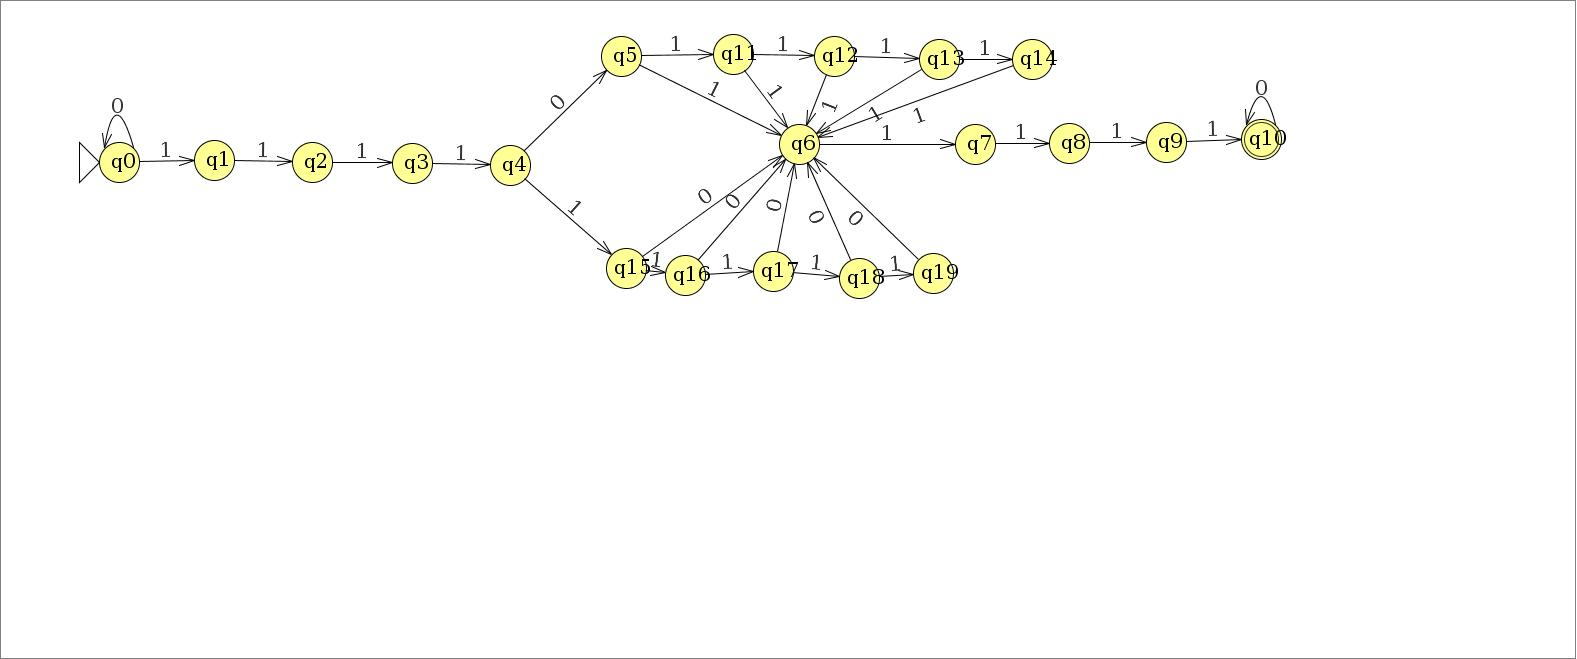
\includegraphics[width=230mm]{./automate.jpg}
\end{center}

Donc, nous avons pour l'automate $A = (\Sigma, Q, q_0, F, T)$.
$$ dom(X_{i,j}) = \Sigma $$

Pour chaque ligne $i$, on cr�e $p + 1$ variables de $Q_{i0}$ ... $Q_{ip}$ avec les domaines,
$$ dom(Q_{i0}) = \{q_0\} $$
$$ dom(Q_{ij}) = Q , \;   0 < j < p $$
$$ dom(Q_{ip}) = F $$

Nous avons les contraintes.
\begin{equation}
Tableau(Q_{i(j-1)},X_{ij},Q_{ij},T)
\end{equation}

\begin{tabular}{ |c|c|c| } 
	\hline
	 & T &  \\
	\hline
	$q_0$ & 0 & $q_0$ \\
	$q_0$ & 1 & $q_1$ \\
	$q_1$ & 1  & $q_2$ \\
	$q_2$ & 1  & $q_3$ \\
	$q_3$ & 1  & $q_4$ \\
	$q_4$ & 0  & $q_5$ \\
	$q_4$ & 1 & $q_{15}$ \\
	$q_5$ & 1 &  $q_{11}$ \\
	$q_5$ & 1 &  $q_{6}$ \\
	$q_6$ & 1 &  $q_7$ \\
	$q_7$ & 1 & $q_8$ \\
	$q_8$ & 1 & $q_9$ \\ 
	$q_9$ & 1 & $q_{10}$ \\
	$q_{10}$ & 0 &  $q_{10}$ \\
	$q_{11}$ & 1 & $q_{6}$\\
	$q_{11}$ & 1 & $q_{12}$\\
	$q_{12}$ & 1 & $q_{6}$\\
	$q_{12}$ & 1 & $q_{13}$\\
	$q_{13}$ & 1 & $q_{6}$\\
	$q_{13}$ & 1 & $q_{14}$\\
	$q_{14}$ & 1 & $q_{6}$\\
	$q_{15}$ & 0 & $q_{6}$\\
	$q_{15}$ & 1 & $q_{16}$\\
	$q_{16}$ & 0 & $q_{6}$\\
	$q_{16}$ & 1 & $q_{17}$\\
	$q_{17}$ & 0 & $q_{6}$\\
	$q_{17}$ & 1 & $q_{18}$\\
	$q_{18}$ & 0 & $q_{6}$\\
	$q_{18}$ & 1 & $q_{19}$\\
	$q_{19}$ & 0 & $q_{6}$\\
	\hline
\end{tabular}


Nous avons utilis� comme heuristique Impact based search avec la coh�rence de bornes et aucun red�marrage. \\ 
\bigskip
La solution retourn�e par le solveur Choco 3: \\
Horaire: \\
  0    0    1    1    1    1    0    1    1    1    1    1    1    1    1    1  \\
  1    1    1    1    1    1    1    0    1    1    1    1    0    0    0    0  \\
  0    0    0    0    1    1    1    1    0    1    1    1    1    1    1    1  \\
  0    1    1    1    1    0    1    1    1    1    1    1    1    0    0    0  \\
  0    0    0    1    1    1    1    0    1    1    1    1    1    1    1    1  \\
Offre: \\
  1    2    3    4    5    4    4    3    4    5    5    5    4    3    3    3  \\
Demande: \\
  1    2    3    4    5    4    2    3    4    3    5    5    4    3    3    3   \\
Perte: \\
  0    0    0    0    0    0   40    0    0   40    0    0    0    0    0    0  \\
\end{document}
